
\documentclass[10pt]{article}
%\usepackage{geometry} % see geometry.pdf on how to lay out the page. There's lots.
%\geometry{a4paper} % or letter or a5paper or ... etc
% \geometry{landscape} % rotated page geometry

% See the ``Article customise'' template for come common customisations
\usepackage{booktabs}

\usepackage{array}

\usepackage{pdflscape}
\usepackage{multirow}
\usepackage{amsmath}
\usepackage{amssymb}
   \usepackage[pdftex]{graphicx}
  % declare the path(s) where your graphic files are
 %  \graphicspath{{./figures/img/}{../jpeg/}}
 \graphicspath{{img/}}

\title{A High Level Constraint Language for  Product Line Enginering}
\author{\'Angela Villota G\'omez}
\date{\today} % delete this line to display the current date

%%% BEGIN DOCUMENT
\begin{document}

\maketitle
%\tableofcontents

\section{HLCL}
HLCL is a constraint-based conceptual modeling language for specifying product line models. A Product Line Model (PLM) defines all the legal combinations of variable artifacts in a product line by means of relationships among them.  Variable artifacts refer to reusable elements that are part of some, but not all, products that can be build from the product line \cite{mazothesis}.

As a conceptual modeling language, HLCL comprises a set of constructs and rules to create PLMs.  The set of constructs and rules is defined by the HLCL grammar.  A collection of statements derived from the HLCL grammar is called a \emph{script}, this script is an specific product line model in HLCL \cite{gemino2004framework}.  Scripts in HLCL are the result of the product line design process and can be obtained either by manual  specification or by automated transformation from existing models. Thus, HLCL can be used as (i) a language to directly specify PLMs, (ii) an intermediate language between product line models and the execution language (iii) a common language to represent a PLM spread in several views, and (iv) a pivot language to represent a product line designed with PLMs in different specification languages.
%On the one hand,  A script is a PLM specification when HLCL is used as a language to create product line models.  On the other hand, a script can be an intermediate representation of a product line model described in other product line notation. 

\begin{figure*}[htb]
\centering
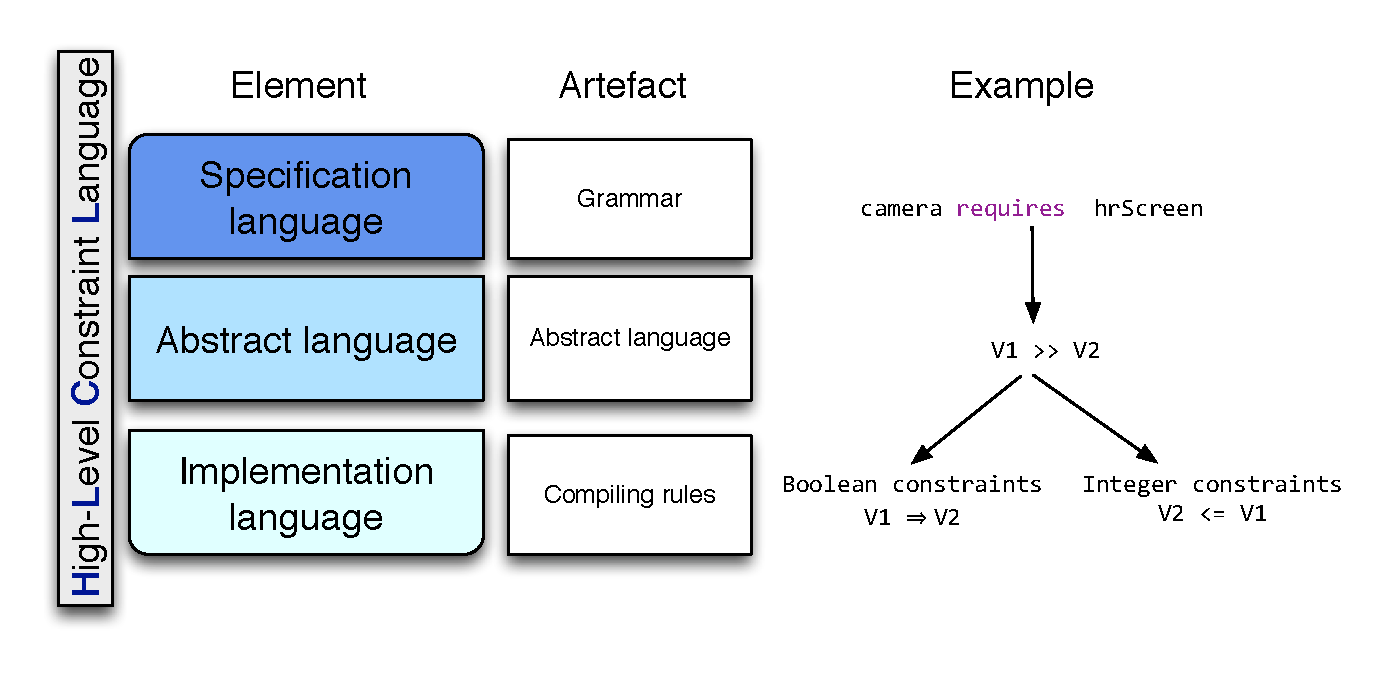
\includegraphics[scale=0.5]{HLCL_overview}
\caption{HLCL Overview}
\label{HLCL_overview}
\end{figure*}

\newpage
\section{Specification Language}
This section describes the grammatical rules to derive product line models in HLCL...
In this section we introduce the grammatical rules for the operations of the HLCL, 
Assuming a set of names $\mathcal{N}$ and
\begin{table}[htb]
\caption{HLCL Grammar}
\label{grammar}
\centering
\begin{tabular}{|lcl|}
\hline
Product line model &&\\
$\langle model\rangle $ 			&$::=$& $\langle identifier\rangle $ $\langle variables\rangle $    $\langle splConstraints\rangle $ \\ 
\hline
Variables and variants&&\\
$\langle variables\rangle $ 		&$::=$& \texttt{`variables:'} $\langle varDeclaration\rangle ^+$  \\
$\langle varDeclaration\rangle $ 	&$::=$& $\langle varType\rangle$ $\langle identifier\rangle$  \texttt{`variants:'} $\langle variantDeclaration\rangle $  \\

$\langle variantDeclaration\rangle $ 	&$::=$&    $\langle variantsInterval\rangle  \mid 
									 \langle variantsEnumeration\rangle $\\ % \mid  las l�neas que siguen son para los 
									 %\langle variantsSet\rangle $  \\	  % conjuntos de variables
$\langle variantsInterval \rangle $ 	&$::=$&  $\langle value \rangle$   \texttt{`::'}  $\langle value\rangle $  \\
$\langle variantsEnumeration\rangle $ &$::=$&  \texttt{`['} $\langle valuesList \rangle$  \texttt{`]'} $\mid$   
									\texttt{`['} $\langle idsList \rangle$  \texttt{`]'} \\
\hline
Constraints&&\\
%$\langle variantsSet\rangle $ 		&$::=$&     \texttt{variants}  \texttt{(} $\langle identifierList \rangle$ \texttt{)} 
%									\texttt{[} $(\langle valuesList \rangle )$   $\{ ,  (\langle valuesList \rangle )\}^*$ \texttt{]}   \\
$\langle splConstraints\rangle $		&$::=$&  \texttt{`constraints:'} $\langle consDefinition\rangle ^+$\\
$\langle consDefinition\rangle$		&$::=$&  $\langle idConstraint\rangle$   \texttt{`:'} $\langle consExpression\rangle $ \\
$\langle consExpression\rangle $	&$::=$& $\langle idConstraint\rangle$  $\mid$
								      $\langle refinement\rangle$ $\mid$
								       $\langle rule\rangle$  $\mid$
								       $\langle foda\rangle$   \\
$\langle refinement\rangle $		&$::=$& $\langle assignment\rangle \mid 
									\langle varRefinement\rangle \mid
									 \langle setRefinement\rangle$  \\
$\langle assignment\rangle $		&$::=$& $\langle identifier\rangle$ \texttt{`is'} $\langle value\rangle$ \\
$\langle varRefinement\rangle$ 	&$::=$& $\langle identifier\rangle$ \texttt{`in'} 
									$\langle variantsInterval \rangle  \mid  
									\langle variantsEnumeration\rangle $\\
$\langle setRefinement\rangle$ 	&$::=$& \texttt{'('} $\langle idsList\rangle$ \texttt{')'}
									\texttt{`variants'}  
									\texttt{`['`('} $\langle valuesList\rangle$ \texttt{`)'} \\
									&& \{ \texttt{`,'`('}  $\langle valuesList\rangle$  \texttt{')'} $\}^+$ \texttt{`]'} \\
$\langle rule\rangle $	&$::=$& $\langle consExpression\rangle$ \texttt{`-->'}  $\langle consExpression\rangle$  \\
$\langle foda\rangle $	&$::=$& $\langle identifier\rangle$ $\langle fodaOP\rangle$ $\langle identifier\rangle$ \\

\hline
Syntactic categories & &\\
$\langle value\rangle $ 			&$::=$&   $\langle integer\rangle \mid$ \texttt{`selected'} $\mid$ \texttt{`unselected'} \\
$\langle varType\rangle $ 			&$::=$&   \texttt{`boolean'} $\mid$ \texttt{`numeric'} \\
$\langle valuesList\rangle $ 		&$::=$&    $\langle value\rangle$ $($\texttt{`,'} $\langle value\rangle )^*$ \\
$\langle idsList\rangle $ 			&$::=$&    $\langle identifier\rangle$ $($\texttt{`,'} $\langle identifier\rangle )^*$ \\
$\langle fodaOp\rangle $			&$::=$&    \texttt{`optional'} $\mid$
									\texttt{`mandatory'} $\mid$
									\texttt{`requires'} $\mid$
									\texttt{`excludes'} \\
$\langle idConstraint\rangle $ 		&$::=$&    \texttt{`C'} $(\langle letter\rangle^* \langle number\rangle^*)^+$\\
\hline
\end{tabular}
\end{table}

\section{Abstract Language}
%A product line model $M$ 
Product line models are defined by a set of variables representing its elements, a set of constraints between these elements and a set of product line predicates. %Let $\mathcal{V}$ a set of variables and $\mathcal{M}$ the set of product line models built on top of $\mathcal{V}$. 
 Thus, a product line model $M$ is defined  by the triplet $M= \langle \mathcal{V},  \mathcal{C}, \mathcal{P}\rangle$ where:

\begin{description}
	\item{$\mathcal{V}$} is the set of variables representing elements in a product line (i.e., requirements, artifacts, parts, etc).
	%\item {$\mathcal{U}$} is the set of unary constraints.  The unary constraint called \emph{includes}  is denoted by $\bullet V_i$.  % meaning all products in the product line contain the element denoted by variable $V_i$
	 \item {$\mathcal{C}$} is the set of constraints. There are two constraints  \emph{requires} and \emph{excludes} denoted by $V_i \gg V_j$ and $V_i \ll V_j$,  respectively.
	  \item {$\mathcal{P}$} is the set of product line predicates.  There are four product line predicates \emph{attribute}, \emph{clone\_at\_least}, \emph{clone\_at\_most}, \emph{clone\_exactly}.
\end{description}

\subsubsection*{Definitions} 
\begin{itemize}
	\item A \emph{product} is a set containing elements in $\mathcal{V}$.
	\item The \emph{domain space}  with respect to $M$, denoted as $S_M$, is a set containing all the products that can be built using the elements in $\mathcal{V}$.  Thus the solution space is equivalent to the power set of  $\mathcal{V}$ without the empty set $\emptyset$ (It is not possible to have a product without elements).  
	  % denoted as  $\mathcal{P}(V) - \emptyset$.
	\item  A \emph{product line} is a set of products specified by a product line model $M$.  All the products in $PL$ are consistent with the constraints and the predicates in $M$. A product line is a proper subset of the \emph{domain space}, $PL \subseteq S_M$. \emph{Note: this may change if we modify the predicates}.
	%represented by the product line model $M$, denoted as $PL_M$ is the set of products  that  are consistent with the constraints in $M$. A product line i $PL$,  which is the set of products in $S$ (the solution space)  that  are consistent with the constraints in $M$.  Thus $PL \subseteq \mathcal{P}(V)$
\end{itemize}

Table \ref{example} presents an example of a product line model with four variables,  two constraints and zero predicates.  The example shows that the product line represented by the product line model contains less products than the domain space.  The following section presents the semantics of the constraints and the predicates.
\begin{table}[htb]
\caption{Example}
\label{example}
\centering
\begin{tabular}{|ccp{10.8cm}|}
\hline
$M$ 			&$=$& $\langle \mathcal{V}, \mathcal{C}, \mathcal{P}\rangle$ \\
$ \mathcal{V}$	&$=$& $\{ V_1, V_2, V_3, V_4\}$\\
%$ \mathcal{U}$	&$=$& $\{ \bullet V_1 \}$\\
$ \mathcal{C}$	&$=$&$\{ V_2 \gg V_4, V_1 \ll V_3 \} $ \\
$ \mathcal{P}$	&$=$&$\{  \} $ \\
$S_M$			&$=$& $\{
%1 
\{V_1\}, 
%2
\{V_2\},
%3
\{V_3\},
%4
\{V_4\},
%5
\{V_1, V_2\},
%6
\{V_1, V_3\},
%7
\{V_1, V_4\},
%8
\{V_2, V_3\},
%9
\{V_2, V_4\},$\\
			& 	& 
%10
$\{V_3, V_4\},
%11
\{V_1, V_2, V_3\},
%12
\{V_1, V_2, V_4\},
%13
\{V_2, V_3, V_4\},
%14
\{V_1, V_3, V_4\},$\\
			& 	& 
%15
$\{V_1, V_2, V_3, V_4\}
\}$\\
$PL$			&$=$& $\{ 
%1
\{V_1\},
%3
\{V_3\},
%4
\{V_4\},
%7
\{V_1, V_4\},
%9
\{V_2, V_4\},$
%10
$\{V_3, V_4\},
%12
\{V_1, V_2, V_4\},
%13
\{V_2, V_3, V_4\}
 \}$\\
\hline
\end{tabular}
\end{table}
%	\item {$\mathcal{R}$} is the set of \emph{requires} constraints between pairs of variables $(V_i, V_j)$.  A requires constraint is denoted by  $V_i \gg V_j$ meaning $V_i$ \textbf{requires} $V_j$.
%	\item {$\mathcal{X}$} is the set of \emph{excludes} constraints between pairs of variables $(V_i, V_j)$. A excludes constraint is denoted by    $V_i \ll V_j$ meaning $V_i$ \textbf{excludes} $V_j$.


\subsection{Variables}
Variables represent elements in a product line. In this representation all the variables represent  reusable elements that are part of some, but not all, products in a product line.  In this sense, variables may or may not be included in a product.  For instance, consider products 
%6
$\{V_1, V_3\}$ and 
%8
$\{V_2, V_3\}$ in table \ref{example}, these products does not contain the variable $V_4$.
  
\subsection{Constraints}
Constraints are relations between variables used to  characterize a  product line. In this sense, the set of products represented by the PLM (e.g., product line $PL$) is  reduced by each constraint.  To explain how each constraint  reduces the set of products in a product line, we first define the projection of a constraint  over the domain space.  Then, we present the definition of product line in terms of the projections of the constraints. Finally, a definition of the semantics of the constraints and predicates is presented. 

Let $M= \langle \mathcal{V}, \mathcal{C}, \mathcal{P}\rangle$  be a product line model with domain space $S_M=  \mathcal{P}( \mathcal{V}) - \emptyset$.

\textbf{Projection of a constraint.} The projection of a constraint $C_i$  over the domain space denoted as $\Pi _{C_i}$ is the set of products $P_i \in S_M$ satisfying the constraint $C_i$.


\textbf{Product line.}
A product line $PL$ is defined as the intersection of all the projections of constraints in the product line model. Let $M= \langle \mathcal{V}, \mathcal{C}, \mathcal{P}\rangle$  be a product line model with constraints  $\mathcal{C} = \{ C_1, C_2, \dots , C_n\}$.  The set of products represented by  $M$ is the product line: \\
 \begin{center}
 $PL: = \Pi_{C_1} \cap \Pi_{C_2}  \cap \dots \cap \Pi_{C_n}$\\
 \end{center}



\subsubsection{Requires}
A requires constraint is a binary relation denoted as $V_i \gg V_j$. If a product line model contains the constraint  $V_i \gg V_j$ then, the inclusion of $V_i$ in a product  implies also the inclusion of  $V_j$.  The requieres constraint is directional, therefore $V_i \gg V_j$ is different than $V_j \gg V_i$. The projection  of $V_i \gg V_j$ is the set of products  $\Pi_{V_i \gg V_j}$ containing all the products in the domain space  that:
 (i) the product contains $V_i, V_j$  at the same time, (ii) the product does not contain  $V_i, V_j$, and (iii) the product contains $V_j$ But does not contain $V_i$.  Let $M= \langle \mathcal{V},  \mathcal{C}, \mathcal{P}\rangle$ be a product line model, with variables $\mathcal{V} = \{V_i, \dots, V_n\}$ and constraints $\mathcal{C} = \{ V_i \gg V_j\}$, the projection $\Pi_{V_i \gg V_j}$ is the set
 \begin{center}
$\Pi_{V_i \gg V_j} = \{ P \mid V_i, V_j \notin P\} \cup  \{ P \mid V_i, V_j \in P \} \cup  \{ P \mid V_i \notin P \land V_j \in P \}  $

\end{center}
Table \ref{requires} presents an example showing how to compute the projection of a requires constraint. 
\begin{table}[htb]
\caption{Example of the requieres semantics}
\label{requires}
\centering
\begin{tabular}{|ccp{7cm} l|}
\hline
$M$ 				&$=$& $\langle \mathcal{V}, \mathcal{C}, \mathcal{P}\rangle$ & product line model \\
$ \mathcal{V}$		&$=$& $\{ V_1, V_2, V_3, V_4\}$& variables\\
%$ \mathcal{U}$	&$=$& $\{ \bullet V_1 \}$\\
$ \mathcal{C}$		&$=$&$\{ V_2 \gg V_4\} $ & constraints\\
$\Pi_{V_2 \gg V_4}$	&$=$& 
$\{	
%9
\{V_2, V_4\},
%12
\{V_1, V_2, V_4\},
%13
\{V_2, V_3, V_4\}, $ & projection\\

 & 	&  
 %15
$\{V_1, V_2, V_3, V_4\} \}  \cup$
 $\{	
%1 
\{V_1\},
%3
\{V_3\},
%6
\{V_1, V_3\},
%%10
%\{V_3, V_4\},
%14
%\{V_1, V_3, V_4\} 
\}  \cup$ &\\

 & 	&  $\{ 
 %4
\{V_4\},
%7
\{V_1, V_4\},
%10
\{V_3, V_4\},
%14
\{V_1, V_3, V_4\} \}  \cup $ & \\

\hline
\end{tabular}
\end{table}

\subsubsection{Excludes}
A excludes constraint is a binary relation denoted as $V_i \ll V_j$.  When the constraint  $V_i \ll V_j$ is included in a product line model, the products 
derived from the product line model cannot contain variables $V_i$ and $V_j$ at the same time.  This constraint  is bi-directional, therefore, $V_i \ll V_j$ is equivalent to $V_j \ll V_i$. The projection  of $V_i \ll V_j$ is the set of products  $\Pi_{V_i \ll V_j}$ containing only the products that does not contain  $V_i, V_j$.  Let $M= \langle \mathcal{V},  \mathcal{C}, \mathcal{P}\rangle$ be a product line model, with variables $\mathcal{V} = \{V_i, \dots, V_n\}$ and constraints $\mathcal{C} = \{ V_i \ll V_j\}$, the projection $\Pi_{V_i \ll V_j}$ is the set
 \begin{center}
$\Pi_{V_i \ll V_j} = \{ P \mid V_i, V_j \notin P\}  $

\end{center}

Table \ref{excludes} presents an example showing how to compute the projection of a excludes constraint. 
\begin{table}[htb]
\caption{Example of the excludes semantics}
\label{excludes}
\centering
\begin{tabular}{|ccp{7cm} l|}
\hline
$M$ 				&$=$& $\langle \mathcal{V}, \mathcal{C}, \mathcal{P}\rangle$ & product line model \\
$ \mathcal{V}$		&$=$& $\{ V_1, V_2, V_3, V_4\}$& variables\\
%$ \mathcal{U}$	&$=$& $\{ \bullet V_1 \}$\\
$ \mathcal{C}$		&$=$&$\{ V_1 \ll V_3\} $ & constraints\\
$\Pi_{V_1 \ll V_3}$	&$=$& 
$\{	
%1 
\{V_1\}, 
%2
\{V_2\},
%3
\{V_3\},
%4
\{V_4\},
%5
\{V_1, V_2\},
%7
\{V_1, V_4\},$ & projection\\
 & 	&  
 %8
 $
\{V_2, V_3\},
 %9
\{V_2, V_4\},
%10
\{V_3, V_4\},
%12
\{V_1, V_2, V_4\},
%13
\{V_2, V_3, V_4\} $ &\\
 

\hline
\end{tabular}
\end{table}

\subsection{Predicates}
Predicates are relations between variables used to represent particular characteristics of such variables. We included in the language a set of predicates to represent relations such as:  composition, and cardinalities.  

\begin{description}
	%\item{Aggregation}
	\item {\textbf{Composition.}} 	
	\begin{enumerate} 
		\item $attribute(a, V)$ to estate that the variable $a$ represents an attribute of $V$.
		\item $parent(V_1, V_2)$ to describe a hierarchical relation between $V_1, V_2$.
	\end{enumerate}
	
	\item{\textbf{Cardinalities.}}
	\begin{enumerate}
		\item $clone\_at\_least(V, a)$ to state that the element represented by a variable $V$ must be cloned at least $a$ times.
		\item $clone\_at\_most(V,a)$  to state that the element represented by a variable $V$ must be cloned at most $a$ times.
		\item $clone\_exactly(V,a)$  to state that the element represented by a variable $V$ must be cloned exactly $a$ times.
		\item  ... other for cardinality n..m
	\end{enumerate}
\end{description}






\subsection{Other variability constraints}
This is a collection of variability constraints and its mapping to HLCL

%%%%%%%%%%%%%%%%%%%%%%%%%%%%%%%%%%%
%%%%%%%%%%%%%%%%%%%%%%%%%%%%%%%%%%%
% variability concepts table


\begin{table*}[h!]
\footnotesize
\caption{Variability constraints mapped to HLCL}
\label{constraints-multiple}
\centering
\small{
\begin{tabular}{ p{2.5cm}p{5.5cm}p{4cm}}
\toprule
Constraint &  Description & HLCL representation  \\
(name in literature) & & \\
\midrule

Excludes  \cite{kang1990feature} & if $V_1$ is present in a product  then $V_2$ must not be present &  $V_1 \ll V_2$ \\
\midrule
Requires  \cite{kang1990feature} & If $V_1$ is present in a product, then $V_2$ must be  present  too & $V_1 \gg V_2$ \\
\midrule
Mandatory  \cite{kang1990feature} & If $V_1$ is present in a product, then $V_2$ must be present as well and vice-versa. &  $V_1 \gg V_2 \land V_2 \gg V_1$\\
\midrule 
Optional \cite{kang1990feature} & If $V_1$ is present in a product $V_2$ may be present, but if  $V_2$ is present, then $V_1$ is present too & $V_2 \gg V_1$ \\
\midrule
\multirow{4}{2.5cm}{Cardinality \cite{czarnecki2005cardinality} Cloning \cite{michel2011formal} }& Let $a$ be an integer.  &\\

	& There are $a$ copies of $V_1$  in the product & $clone\_exactly(V_1, a)$ \\ 
	\cmidrule{2-3}
	& There are  at least $a$ copies of $V_1$  in the product & $clone\_at\_least(V_1, a)$ \\ 
	\cmidrule{2-3}
	& There are at most  $a$ copies of $V_1$  in the product & $clone\_at\_most(V_1, a)$ \\ 
\midrule
\multirow{2}{2.5cm}{Attributes \cite{czarnecki2005cardinality,benavides2005automated}, Non-functional features \cite{kang1998form} } & Let  $a_1, \dots , a_n$ be variables representing attributes of $V$. & \\
& If $V$ is present in a product, then all its attributes are present in the product. & $(attribute(a_1, V) \land \dots \land attribute(a_n, V)) \land ( V \gg a_1 \land \dots \land V \gg a_n) \land (a_1..a_n \gg V)$	\\



\bottomrule
\end{tabular}
}
\end{table*}


\newpage
\bibliographystyle{plain}
%\bibliographystyle{IEEEabrv}
 \bibliography{../hlcl}
\end{document}